不同编程语言的执行模型也不同,最常见的便是解释语言和编译语言。编译器将源代码翻译成机器代码,计算机可以在没有中间系统支持的环境下运行。另外,解释性语言代码需要支持系统、解释器和虚拟环境才能工作。 \par
C++是编译语言,所以会比解释型程序运行得更快。但C++程序需要针对每个平台进行编译,但解释型程序可以跨平台运行。 \par
我们将讨论程序构建的细节,从源代码阶段开始——由编译器完成——到可执行文件(编译器的输出)结束。还会去了解,为什么为一个平台构建的程序不能在另一个平台上运行。 \par
本章将讨论以下主题: \par

\begin{itemize}
	\item 介绍C++20。
	\item C++预处理的细节。
	\item 源代码的(底层)编译。
	\item 了解连接器及其功能。
	\item 加载和运行可执行文件的过程。
\end{itemize}

\noindent\textbf{}\ \par
\textbf{技术要求} \\
g++编译器需要添加编译选项 \texttt{-std=c++2a} 来编译本章的代码。可以从这里获取本章的源码文件:https:/​/github.​com/PacktPublishing/Expert-CPP \par

\noindent\textbf{}\ \par
\textbf{介绍C++20} \\
C++经过多年的发展,目前发展到C++ 20。自C++ 11以来,C++标准已经对语言的特性集进行了极大地扩展。现在,让我们来看看C++ 20标准中哪些值得关注的特性。 \par

\noindent\textbf{}\ \par
\textbf{概念(Concepts):}\ \par
概念是C++ 20的主要特性之一,它为类型提供了一组需求。概念的基本思想是模板参数的编译时进行验证,例如:要指定模板实参必须有默认构造函数,可以使用\textbf{default\underline{ }constructible}概念,方法如下: \par
\noindent\textbf{}\ \par

	%template <\textbf{default\underline{ }constructible} T> \par
	%void make\underline{ }T() { return T(); } \par
	
\begin{lstlisting}[caption={}]
template <default_constructible T>
void make_T() { return T(); }
\end{lstlisting}
	
\noindent\textbf{}\ \par
上面的代码中,我们忽略了typename关键字,设置一个概念来描述模板函数的形参T。\par

可以说概念是描述其他类型的类型——可称为元类型。允许在编译时验证模板参数,以及基于类型属性的函数调用。我们将在第3章和第4章中详细讨论这些概念。 \par

\noindent\textbf{}\ \par
\textbf{协程(Coroutines):}\ \par
协程是能够在执行点停止,并在稍后恢复的特殊函数。协程用以下关键字进行扩展:\par

\begin{enumerate}
	\item \texttt{co\underline{ }await} 暂停协程的执行。
	\item \texttt{co\underline{ }yield} 暂停协程的执行,同时返回一个值。
	\item \texttt{co\underline{ }return} 类似于return,完成协程时返回一个值。举个栗子:
\end{enumerate}

%	generator<int> step\underline{ }by\underline{ }step(int n = 0) \{ \par
%		\quad while (true) \{ \par
%			\quad \quad \textbf{co\underline{ }yield} n++; \par
%		\quad \} \par
%	\} \par

\begin{lstlisting}[caption={}]
generator<int> step_by_step(int n = 0) {
	while (true) {
		co_yield n++;
	}
}
\end{lstlisting}

\noindent\textbf{}\ \par
协程与promise对象相关联,promise可以存储协程的状态并发出警报。我们将在第8章中更深入地研究协程。 \par
	
\noindent\textbf{}\ \par
\textbf{范围(Ranges):}\ \par
范围库提供了一种处理元素范围的新方法。要使用它们,首先要包含<ranges>头文件。来看一个例子,范围是一个有开始和结束的元素vector,提供了一个begin迭代器和一个end哨兵:\par

\begin{lstlisting}[caption={}]
import <vector>
int main()
{
	std::vector<int> elements{0, 1, 2, 3, 4, 5, 6};
}
\end{lstlisting}

带有范围适配器(\texttt{|}操作符)的范围支持处理一系列元素的功能。看下代码: \par

\begin{lstlisting}[caption={}]
import <vector>
import <ranges>
int main()
{
	std::vector<int> elements{0, 1, 2, 3, 4, 5, 6};
	for (int current : elements | ranges::view::filter([](int e) { return
		e % 2 == 0; }))
	{
		std::cout << current << " ";
	}
}
\end{lstlisting}

前面的代码中,使用\texttt{ranges::view::filter()}过滤偶数。请注意\texttt{|}可以在不同的vector间使用。我们将在第7章中讨论范围及其强大的特性。 \par

\noindent\textbf{}\ \par
\textbf{更多C++20的特性}\ \par
C++ 20是一个大版本,它包含了许多更加复杂和灵活的特性。概念、范围和协程是本书讨论的众多特性中部分。 \par
最受期待的特性(之一)是模块,它提供了声明模块,以及在这些模块中导出类型和值的能力。可以将模块视为带有包含保护头文件,也就是头文件的改进版本。本章将介绍C++20中模块的特性。 \par
除了C++ 20中添加的一些特性外,我们还将在本书中讨论其他一些特性: \par

\begin{itemize}
	\item 超级操作符: \texttt{operator<=>()}。 现在可以利用\texttt{<=>()}来控制操作符重载的冗长程度。
	\item \texttt{constexpr}在这门语言中越来越常见。C++ 20现在添加了\texttt{consteval}函数、\texttt{constexpr std::vector}和\texttt{std::string}等类型。
	\item 数学常量,如\texttt{std::number::pi}和\texttt{std::number::log2e}。
	\item 线程库的更新,包括停止令牌和加入线程。
	\item 概念迭代器。
	\item 仅移动视图和其他功能。
\end{itemize}

为了更好地理解一些新特性并深入到该语言的本质,我们将从以前的版本开始介绍该语言的核心。这将有助于我们找到新特性相对于旧特性的更好用法,也将有助于支持历史遗留的C++代码。现在让我们从理解C++应用程序的构建开始。 \par

\noindent\textbf{}\ \par
\textbf{构建并运行程序}\ \par
可以使用任何文本编辑器来编写代码,因为代码就是文本。可以在简单的文本编辑器(如Vim)和高级集成开发环境(IDE)(如MS Visual Studio)之间自由选择。情书和源代码的唯一区别是后者可能由一种称为编译器的特殊程序解释(虽然情书不能被编译成程序,但它可能会让你紧张不安)。\par
为了区分文本文件和源代码,使用文件扩展名对二者进行区分。C++源码文件扩展为.cpp和.h(可能偶尔也会遇到.cxx和.hpp)。在讨论细节之前,请将编译器视为一种将源代码转换为可运行程序(即可执行文件)的工具,而源代码生成可执行文件的过程称为编译。编译C++程序是生成机器码的一系列复杂任务,机器码是计算机可以看得懂的语言。 \par
通常,C++编译器会解析和分析源码,然后生成中间码,对其进行优化,最后在目标文件中生成机器码。读者们可能见过目标文件了,它们有各自的扩展名,Linux中的.o和Windows中的.obj。所创建的目标文件不仅包含计算机可以运行的机器码,编译通常涉及几个源文件,编译每个源文件会生成一个目标文件。然后,这些目标文件通过链接器链接在一起,形成一个的可执行文件。链接器使用存储在目标文件中的附加信息,来正确地链接它们(链接将在本章后面讨论)。 \par
下面的图表描述了程序构建各个阶段: \par

\begin{center}
	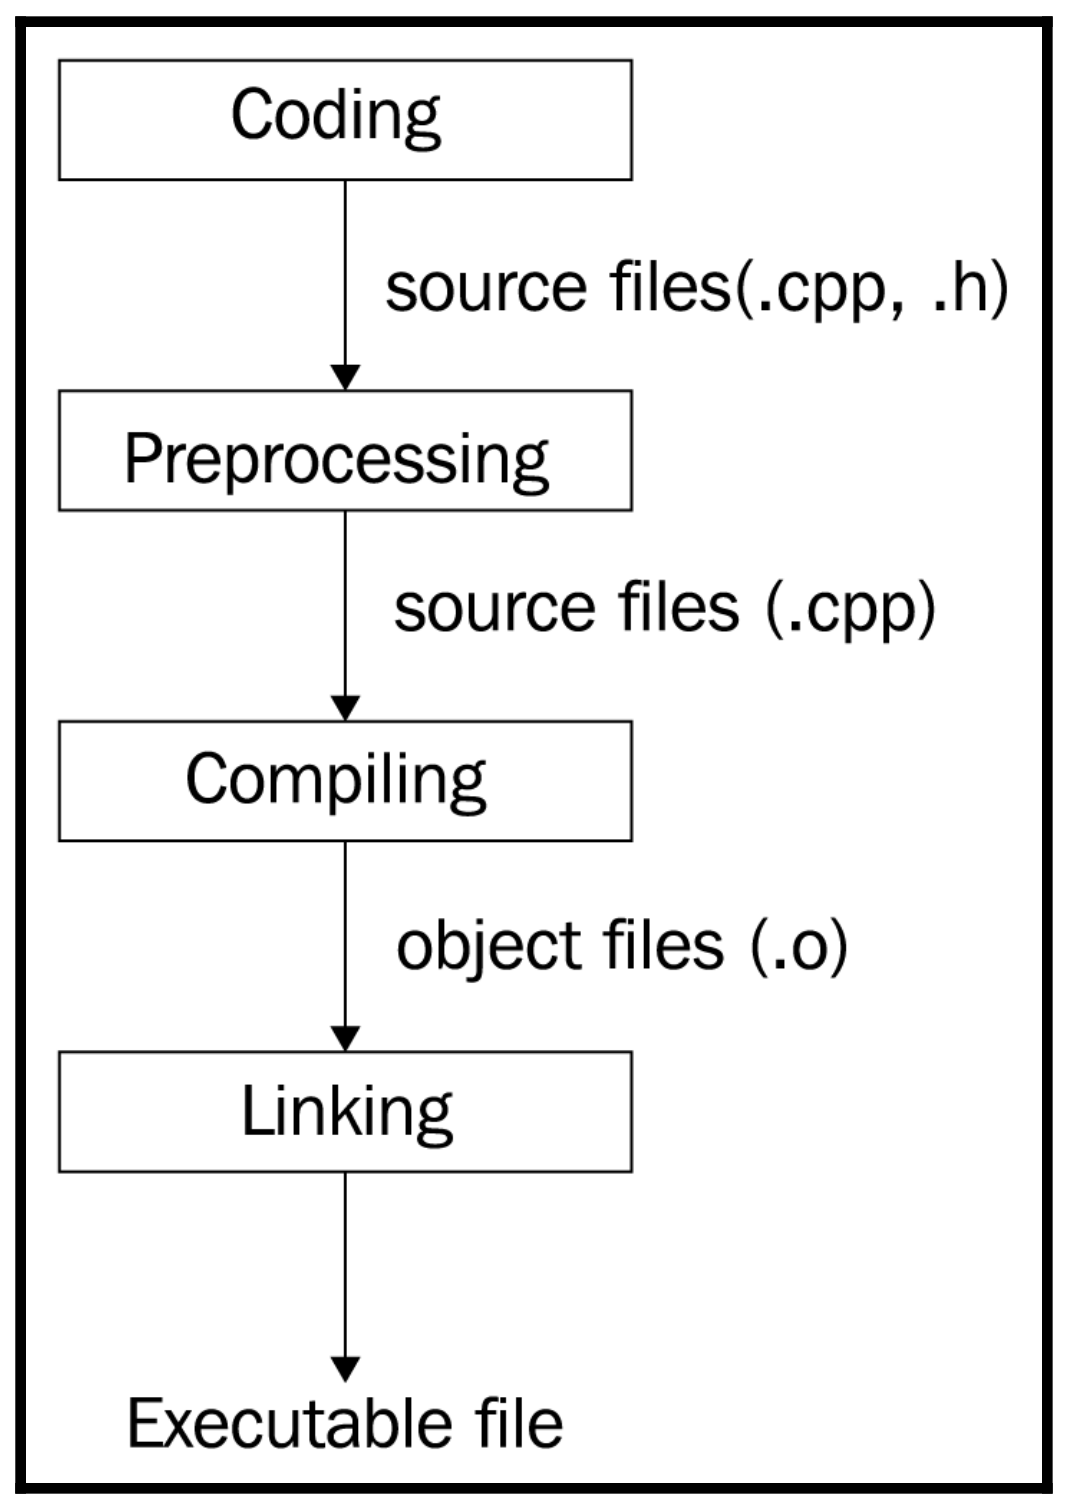
\includegraphics[width=0.3\textwidth]{content/Section-1/Chapter-1/1}
\end{center}

C++应用程序构建过程包括三个主要步骤:预处理、编译和链接。这些步骤使用不同的工具完成,但是编译器将它们封装在一个工具中,从而为程序员提供了更直接的接口。\par
生成的可执行文件保存在计算机的硬盘驱动器上,运行时会复制到主存RAM中,复制是由另一个名为加载器的工具完成。加载器是操作系统的一部分,它知道应该从可执行文件的内容中复制什么内容,以及在哪里复制。并且,加载的可执行文件不会从硬盘上删除。 \par
程序的加载和运行由操作系统(OS)完成,操作系统管理程序的执行,先执行优先级高的程序,完成后卸载程序等工作。程序的运行副本称为进程,进程是可执行文件的实例。 \par

\noindent\textbf{}\ \par
\textbf{预处理}\ \par
预处理器对源文件进行处理,使它们为编译做好准备。预处理器使用预处理器指令,比如\#define、\#include等等。指令不代表程序语句,但它们是预处理命令,告诉预处理器如何处理源文件的文本。编译器无法识别这些指令,因此无论何时在代码中使用预处理器指令,预处理器都会在代码开始实际编译之前解析它们。例如,以下代码将在编译器开始编译之前修改:\par

\begin{lstlisting}[caption={}]
#define NUMBER 41
int main() {
	int a = NUMBER + 1;
	return 0;
}
\end{lstlisting}

使用\#define指令是的定义称为宏。经过预处理后,编译器得到转换后的源文件如下: \par

\begin{lstlisting}[caption={}]
int main() {
	int a = 41 + 1;
	return 0;
}
\end{lstlisting}

预处理程序只处理文本,不关心语言规则或语法。使用预处理器指令,特别是宏定义,如前面的例子中,\#define NUMBER 41很容易出错,除非预处理器只是简单地将NUMBER替换为41,而没有将41解释为整数。对于预处理器,以下两行都是有效的:\par

\begin{lstlisting}[caption={}]
int b = NUMBER + 1;
struct T {}; // user-defined type
T t = NUMBER; // preprocessed successfully, but compile error
\end{lstlisting}

预处理后的代码: \par

\begin{lstlisting}[caption={}]
int b = 41 + 1
struct T {};
T t = 41; // error line
\end{lstlisting}

编译器开始编译时,发现t = 41是错误的,因为没有从'int'到' T'的转换。\par
使用语法正确,但有逻辑错误的宏非常危险: \par

\begin{lstlisting}[caption={}]
#define DOUBLE_IT(arg) (arg * arg)
\end{lstlisting}

预处理器将用(arg * arg)替换任何出现的DOUBLE\underline{}IT(arg),因此下面的代码将输出16: \par

\begin{lstlisting}[caption={}]
int st = DOUBLE_IT(4);
std::cout << st;
\end{lstlisting}

编译器接收到的代码如下所示: \par

\begin{lstlisting}[caption={}]
int st = (4 * 4);
std::cout << st;
\end{lstlisting}

当使用复杂表达式作为宏的参数时,会出现问题: \par

\begin{lstlisting}[caption={}]
int bad_result = DOUBLE_IT(4 + 1);
std::cout << bad_result;
\end{lstlisting}

这段代码期望输出25,但预处理程序除了文本处理之外什么都不做,所以会像这样替换宏:\par

\begin{lstlisting}[caption={}]
int bad_result = (4 + 1 * 4 + 1);
std::cout << bad_result;
\end{lstlisting}

输出是 9 ,而不是期望的25。 \par
对宏定义进行修正,需要在宏参数周围加上括号:\par

\begin{lstlisting}[caption={}]
#define DOUBLE_IT(arg) ((arg) * (arg))
\end{lstlisting}

现在预处理后的代码如下: \par

\begin{lstlisting}[caption={}]
int bad_result = ((4 + 1) * (4 + 1));
\end{lstlisting}

强烈建议在合适的情况下使用const声明,而非宏定义。 \par

\hspace*{\fill} \\ %插入空行

\includegraphics[width=0.05\textwidth]{images/tip}
经验法则:避免使用宏定义。宏易于出错,C++提供的构造方式可以不使用宏。 \par

\noindent\textbf{}\ \par
如果使用constexpr函数,则会在编译时检查类型并处理,使用上例: \par

\begin{lstlisting}[caption={}]
constexpr int double_it(int arg) { return arg * arg; }
int bad_result = double_it(4 + 1);
\end{lstlisting}

使用constexpr说明符可以在编译时计算函数的返回值(或变量的值)。有数字定义的例子最好使用const变量: \par

\begin{lstlisting}[caption={}]
const int NUMBER = 41;
\end{lstlisting}

\noindent\textbf{}\ \par
\textbf{头文件}\ \par
预处理器最常见的用法是\#include指令,用于在源代码中包含头文件。头文件包含函数、类等定义: \par

\begin{lstlisting}[caption={}]
// file: main.cpp
#include <iostream>
#include "rect.h"
int main() {
	Rect r(3.1, 4.05)
	std::cout << r.get_area() << std::endl;
}
\end{lstlisting}

假设头文件rect.h的定义如下: \par

\begin{lstlisting}[caption={}]
// file: rect.h
struct Rect
{
	private:
	double side1_;
	double side2_;
	public:
	Rect(double s1, double s2);
	const double get_area() const;
};
\end{lstlisting}

包含在rect.cpp中: \par

\begin{lstlisting}[caption={}]
// file: rect.cpp
#include "rect.h"
Rect::Rect(double s1, double s2)
: side1_(s1), side2_(s2)
{}
const double Rect::get_area() const {
	return side1_ * side2_;
}
\end{lstlisting}

预处理器检查main.cpp和rect.cpp之后,其会将\#include替换为相应的iostream头文件中的内容,并将rect.h的内容替换到main.cpp和rect.cpp中。C++17 引入了\underline{~~}has\underline{ }include 预处理常量表达式。 \underline{~~}has\underline{ }include如果找到指定名称的文件,则计算结果为1,否则为0: \par

\begin{lstlisting}[caption={}]
#if __has_include("custom_io_stream.h")
#include "custom_io_stream.h"
#else
#include <iostream>
#endif
\end{lstlisting}

声明头文件时,强烈建议使用包含保护(include-guards) (\#ifndef, \#define, \#endif)方式,以避免多重声明。同样,这些也是预处理器指令,以避免以下情况:\par

\begin{lstlisting}[caption={}]
// file: square.h
#include "rect.h"
struct Square : Rect {
	Square(double s);
};
\end{lstlisting}

在main.cpp中同时包含square.h和rect.h会导致包含rect.h两次: \par

\begin{lstlisting}[caption={}]
// file: main.cpp
#include <iostream>
#include "rect.h"
#include "square.h"
/*
	preprocessor replaces the following with the contents of square.h
*/
// code omitted for brevity
\end{lstlisting}

预处理后,编译器将接收到如下的main.cpp: \par

\begin{lstlisting}[caption={}]
// contents of the iostream file omitted for brevity
struct Rect {
	// code omitted for brevity
};
struct Rect {
	// code omitted for brevity
};
struct Square : Rect {
	// code omitted for brevity
};
int main() {
	// code omitted for brevity
}
\end{lstlisting}

然后,编译器将报出一个错误,因为它遇到了两个Rect类型的声明。头文件应该通过以下方式使用包含保护来防止多重包含: \par

\begin{lstlisting}[caption={}]
#ifndef RECT_H
#define RECT_H
struct Rect { ... }; // code omitted for brevity
#endif // RECT_H
\end{lstlisting}

当预处理器第一次遇到头文件时,RECT\underline{ }H没有定义,在\#ifndef和\#endif之间的语句都会进行处理,包括RECT\underline{ }H的定义。当预处理器第二次在同一源文件中包含同一头文件时,因为RECT\underline{ }H已经定义,所以会省略其中的内容。 \par
包含保护是控制源文件部分编译的指令的一部分。所有的条件编译指令为\#if、\#ifdef、\#ifndef、\#else、\#elif和\#endif。\par
条件编译在许多情况下非常有用,可以在调试模式下记录函数调用。在发布程序之前,建议对程序进行调试,并针对逻辑缺陷进行测试。你可能想看看调用某个函数后代码中会发生什么,例如: \par

\begin{lstlisting}[caption={}]
void foo() {
	log("foo() called");
	// do some useful job
}
void start() {
	log("start() called");
	foo();
	// do some useful job
}
\end{lstlisting}

每个函数会调用log()函数,其实现如下: \par

\begin{lstlisting}[caption={}]
void log(const std::string& msg) {
#if DEBUG
	std::cout << msg << std::endl;
#endif
}
\end{lstlisting}

如果定义了DEBUG, log()函数将打印msg。如果你编译的项目启用了DEBUG(使用编译器标记,例如\texttt{g++}中的\texttt{-D}),那么log()函数将打印传递给它的字符串,否则什么都不做。 \par

\noindent\textbf{}\ \par
\textbf{C++20中的模块}\ \par
模块避免了头文件中恼人的包含保护问题,现在可以摆脱预处理宏。模块包含有两个相关的关键字,import和export。要使用一个模块,我们需要import。要声明带有导出属性的模块,我们使用export。在列出模块的好处前,先看一个简单的使用示例。下面的代码声明了一个模块: \par

\begin{lstlisting}[caption={}]
export module test;
export int twice(int a) { return a * a; }
\end{lstlisting}

第一行声明了名为test的模块。接下,声明twice()函数,并将其设置为export。这意味着可以也有未导出的函数和其他实例,这些未导出的部分是模块私有的。通过导出,可以将其设置为模块的公共部分。要使用模块,可参照下面的代码: \par

\begin{lstlisting}[caption={}]
import test;
int main()
{
	twice(21);
}
\end{lstlisting}

模块是C++中一个期待已久的特性,它在编译和维护方面提供了更好的性能。以下特性使模块比常规头文件的表现得更好:\par

\begin{itemize}
	\item 一个模块只导入一次,类似于自定义语言实现所支持的预编译头文件。这大大减少了编译时间。未导出的元素对导入模块的单元没有影响。
	\item 模块允许选择哪些单元导出,哪些不导出,从而表达代码的逻辑。模块可以绑定到更大的模块中。
	\item 摆脱前面描述的包含安全之类的工作区。可以以任何顺序导入模块,不再需要考虑宏的重新定义。
\end{itemize}

\noindent\textbf{}\ \par
模块可以与头文件一起使用。我们可以在同一个文件中导入和包含头文件,如下面的例子所示: \par

\begin{lstlisting}[caption={}]
import <iostream>;
#include <vector>
int main()
{
	std::vector<int> vec{1, 2, 3};
	for (int elem : vec) std::cout << elem;
}
\end{lstlisting}

创建模块时,可以自由地导出模块接口文件中的元素,并将实现移动到其他文件中。逻辑与管理的方式.h和.cpp文件相同。 \par

\noindent\textbf{}\ \par
\textbf{编译阶段}\ \par
C++编译过程包括几个阶段。其中一些阶段用于分析源代码,其他阶段用于生成和优化目标机器代码。下面的图表显示了编译的阶段:\par

\begin{center}
	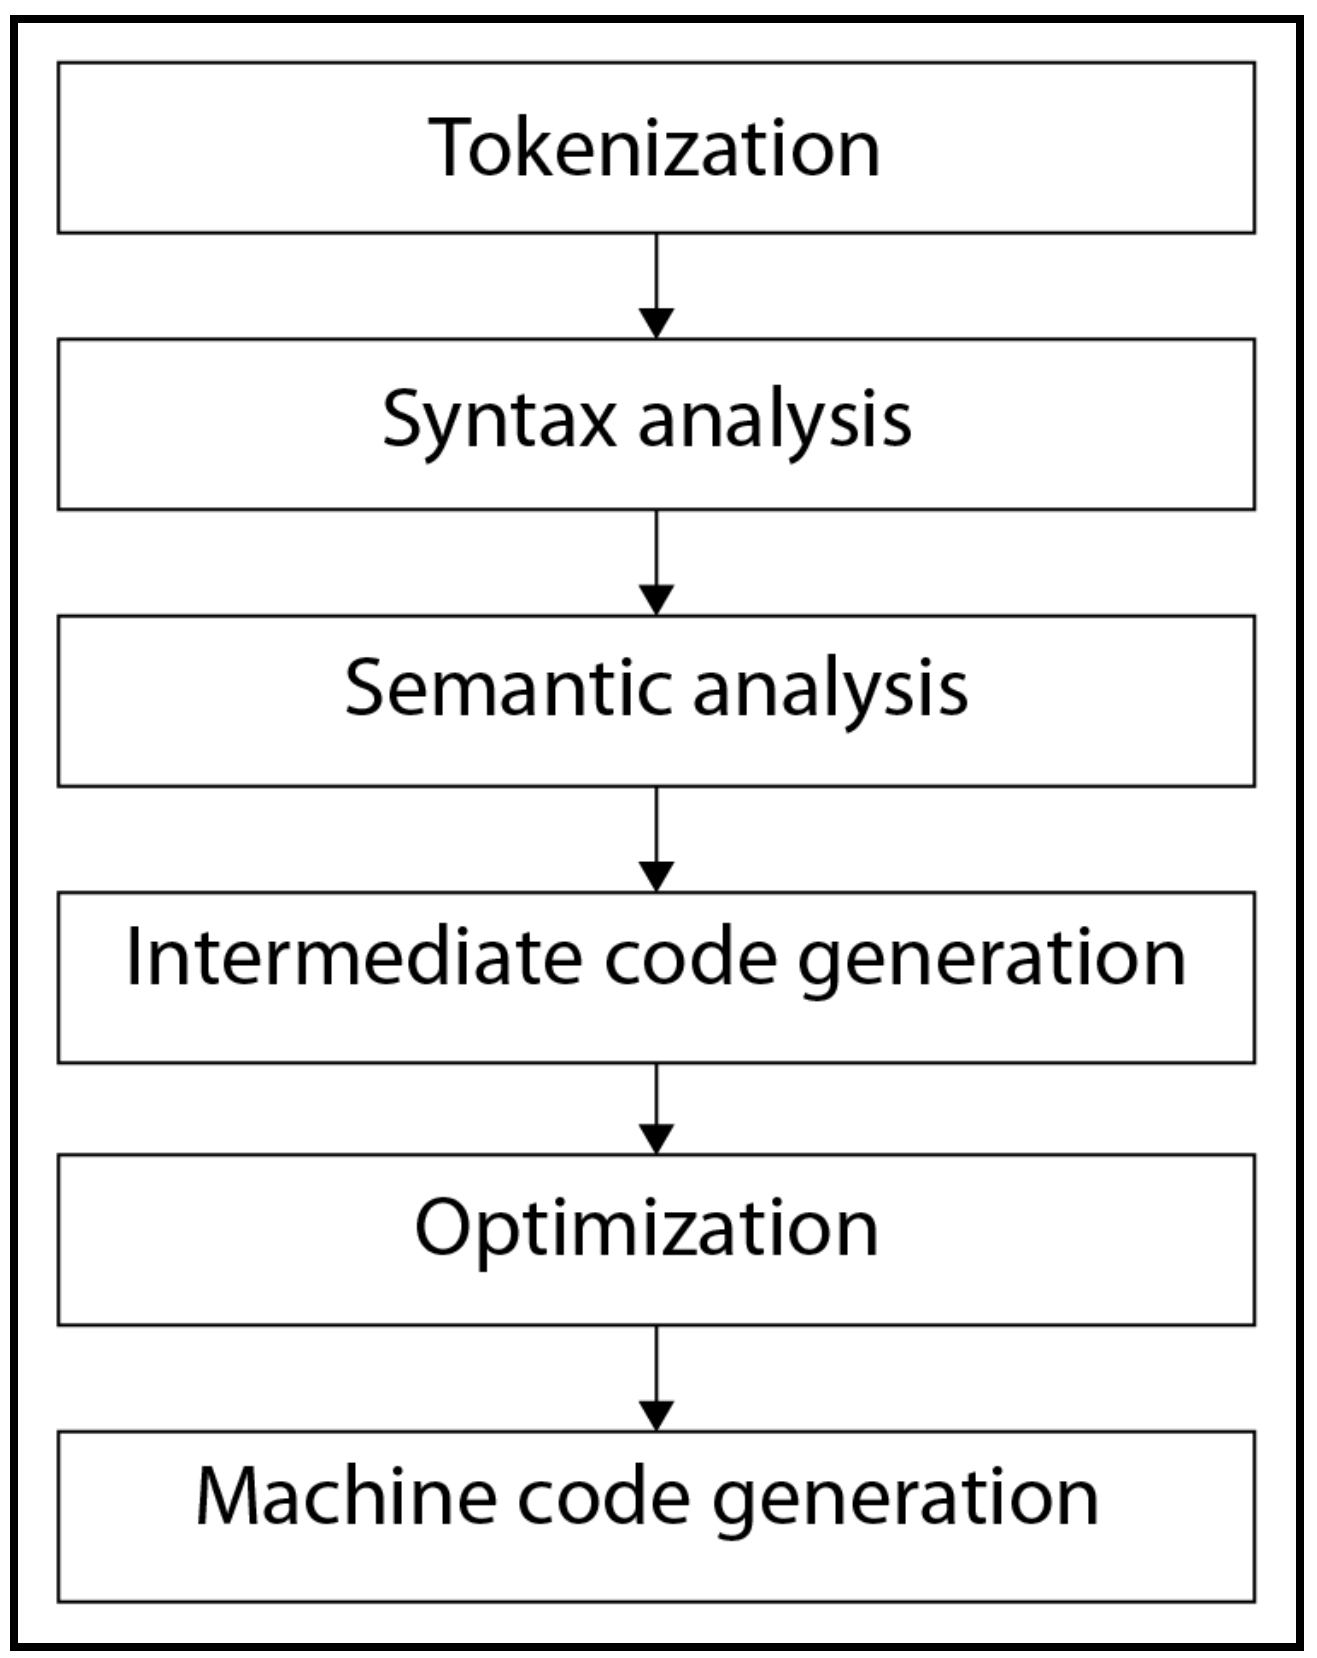
\includegraphics[width=0.3\textwidth]{content/Section-1/Chapter-1/2}
\end{center}

让我们详细地来了解每一个阶段。 \par

\noindent\textbf{}\ \par
\textbf{符号化}\ \par
编译器的分析阶段旨在将源代码分割成可符号化的小单元。一个符号可以是一个单词,也可以只是一个操作符,比如=(等号)。符号是源代码中的原子单元,为编译器带来有意义的值,例如:表达式\texttt{int a = 42;}将被分为符号\texttt{int, a, =, 42,;}。表达式不用空格分隔,下面的表达式也会分割成相同的标记(但建议不要忘记操作数之间的空格): \par

\begin{lstlisting}[caption={}]
int a=42;
\end{lstlisting}
	
使用正则表达式的复杂方法,将源码分割成符号的,这个过程称为“词法分析”,或“符号化”(分为符号)。对于编译器来说,使用符号化的输入,是构建用于分析代码语法的内部数据结构的更好方法。 \par
	
\noindent\textbf{}\ \par
\textbf{语法分析}\ \par	
当谈到编程语言的编译时,我们通常区分两个术语:语法和语义。语法是代码的结构,定义了符号组合结构的规则,例如:\texttt{day nice}在英语中是一个语法正确的短语,因为它的任何一个标记都不包含错误。另外,语义关注的是代码的实际意义,也就是说\texttt{day nice}在语义上是不正确的,应该改为\texttt{a nice day}。\par	
语法分析是源码分析的关键部分,即使符号符合一般语法规则,也要对其进行语法和语义分析。以下代码为例: \par

\begin{lstlisting}[caption={}]
int b = a + 0;
\end{lstlisting}	
	
这对我们来说可能没有意义,因为向变量添加0不会改变它的值,但编译器并不寻找逻辑意义——它寻找代码的语法正确性(缺少分号、缺少闭括号等)。编译的语法分析阶段检查代码的语法正确性。词法分析将代码分成符号,语法分析检查符号语法的正确性。如果我们遗漏了一个分号,上述表达式将产生语法错误: \par

\begin{lstlisting}[caption={}]
int b = a + 0
\end{lstlisting}	
	
g++将会报出一个错误:\texttt{expected ';' at end of declaration}。 \par
	
\noindent\textbf{}\ \par
\textbf{语义分析}\ \par	
如果前面的表达式是这样的\texttt{b = a + 0;}时,编译器将把它分成标记为it、b、=和其他。我们知道有些是未知的,但对编译器来说,这是没问题的。不过,这将导致在g++中的编译错误\texttt{ unknown type name "it" }。寻找表达式背后的含义,才是语义分析(解析)的任务。 \par

\noindent\textbf{}\ \par
\textbf{生成中间码}\ \par	
所有的分析完成后,编译器会生成中间码,这是一个阉割的C++,主要是由C语言构成。一个简单的例子如下: \par	

\begin{lstlisting}[caption={}]
class A {
	public:
	int get_member() { return mem_; }
	private:
	int mem_;
};
\end{lstlisting}	

对代码进行分析之后,将生成中间码(这是一个抽象的例子,意在展示中间代码生成的思想,编译器可能在实现上有所不同):\par	

\begin{lstlisting}[caption={}]
struct A {
	int mem_;
};
int A_get_member(A* this) { return this->mem_; }
\end{lstlisting}

\noindent\textbf{}\ \par
\textbf{优化}\ \par	
生成中间码有助于编译器在代码中进行优化,编译器可以优化代码。优化是在多次转换中完成的,例如下面的代码: \par

\begin{lstlisting}[caption={}]
int a = 41;
int b = a + 1;
\end{lstlisting}

在编译过程中,将被优化为: \par

\begin{lstlisting}[caption={}]
int a = 41;
int b = 41 + 1;
\end{lstlisting}

再次优化为: \par

\begin{lstlisting}[caption={}]
int a = 41;
int b = 42;
\end{lstlisting}

一些程序中,如今的编译器比程序员代码写得更好。 \par

\noindent\textbf{}\ \par
\textbf{生成机器码}\ \par	
编译器优化是在中间码和生成的机器码中完成的。当我们编译这个项目的时候是什么样子的呢?之前,当我们讨论源代码的预处理时,看了一个包含几个源文件的简单结构,包括两个头文件,rect.h和square.h,每个头文件都有它的.cpp文件,以及main.cpp包含程序入口点(main()函数)。预处理之后,下面的单元是编译器的输入为:main.cpp, rect.cpp和square.cpp,如下图所示: \par	

\begin{center}
	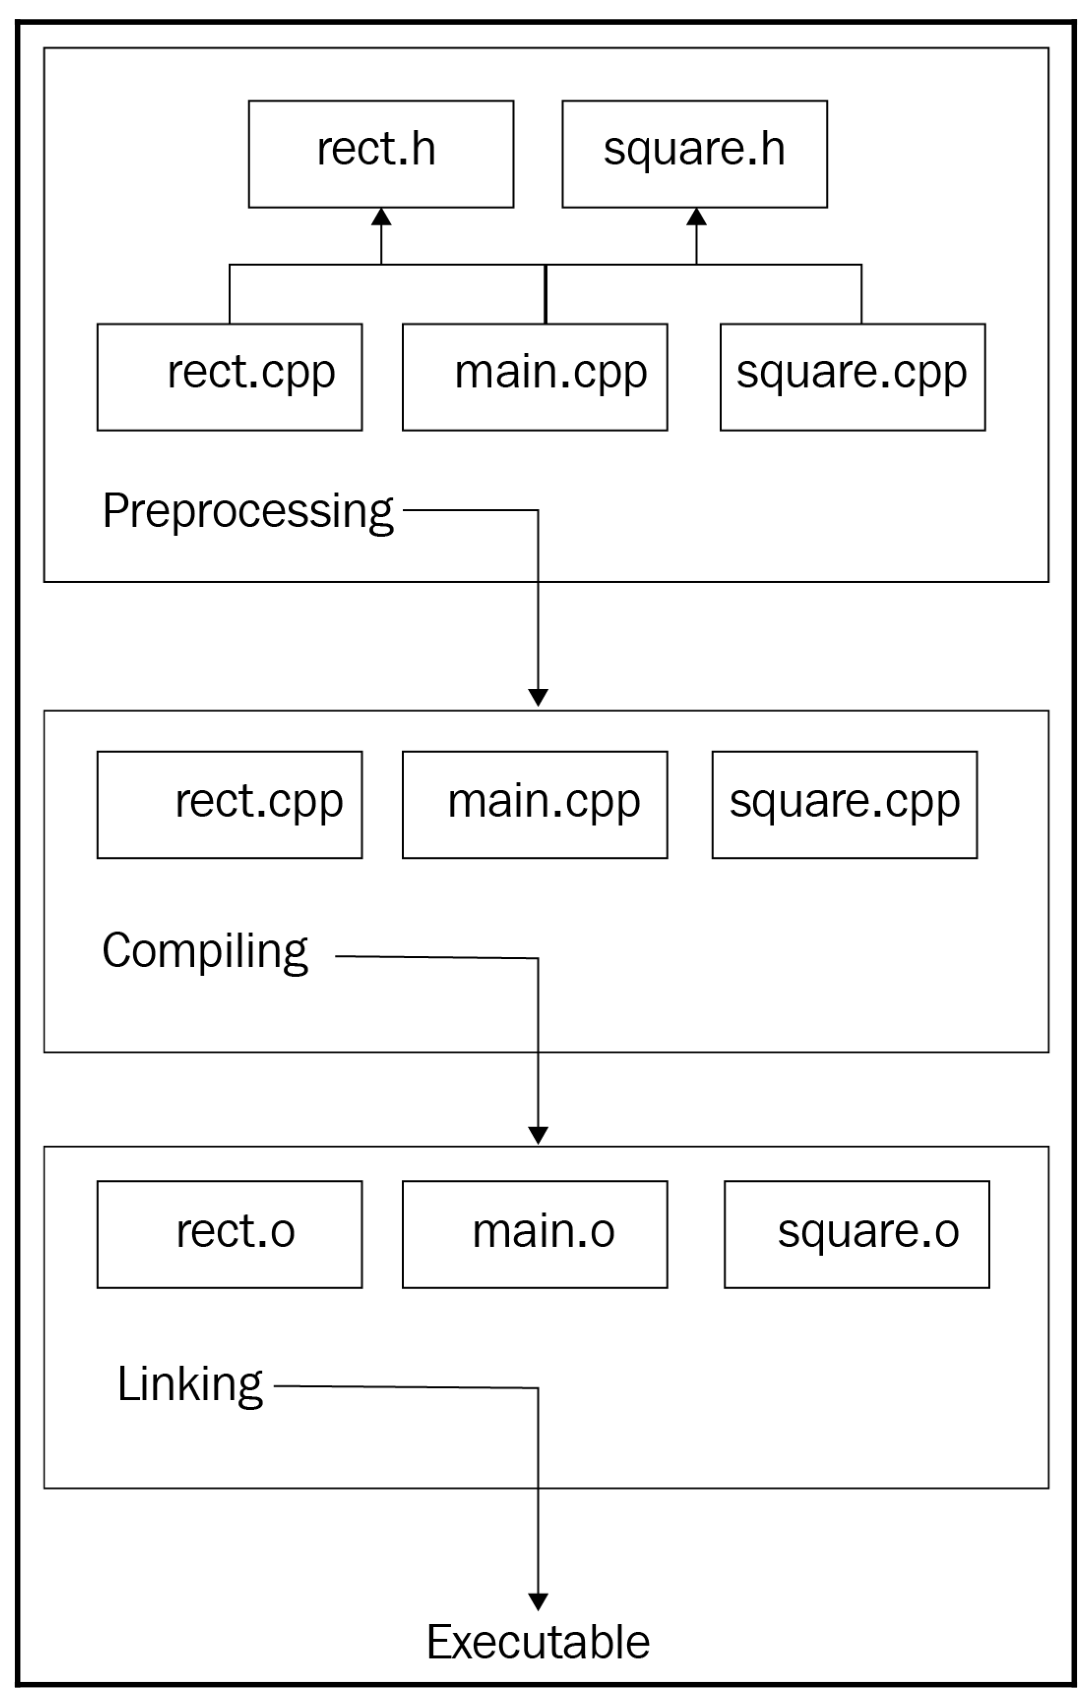
\includegraphics[width=0.3\textwidth]{content/Section-1/Chapter-1/3}
\end{center}

编译器将分别编译。编译单元,也称为源文件,在某种程度上彼此独立。当编译器编译在Rect中调用get\underline{ }area()函数的main.cpp时,不包含main.cpp中的get\underline{ }area()实现。相反,它只能确定该功能是在项目的某个地方实现的。当编译器到达rect.cpp时,编译器并不知道get\underline{ }area()函数在哪里使用。\par
下面是编译器在main.cpp通过预处理阶段后得到的结果: \par

\begin{lstlisting}[caption={}]
// contents of the iostream
struct Rect {
	private:
	double side1_;
	double side2_;
	public:
	Rect(double s1, double s2);
	const double get_area() const;
};
struct Square : Rect {
	Square(double s);
};
int main() {
	Rect r(3.1, 4.05);
	std::cout << r.get_area() << std::endl;
	return 0;
}
\end{lstlisting}

分析main.cpp之后,编译器生成如下中间码(为了简单地表达编译的思想,省略了很多细节): \par

\begin{lstlisting}[caption={}]
struct Rect {
	double side1_;
	double side2_;
};
void _Rect_init_(Rect* this, double s1, double s2);
double _Rect_get_area_(Rect* this);
struct Square {
	Rect _subobject_;
};
void _Square_init_(Square* this, double s);
int main() {
	Rect r;
	_Rect_init_(&r, 3.1, 4.05);
	printf("%d\n", _Rect_get_area(&r));
	// we've intentionally replace cout with printf for brevity and
	// supposing the compiler generates a C intermediate code
	return 0;
}
\end{lstlisting}

编译器在优化代码时将删除Square结构体,及其构造函数(我们将其命名为\underline{ }Square\underline{ }init\underline{ }),因为它从未在源代码中使用过。 \par
此时,编译器只操作main.cpp,因此看到调用了\underline{ }Rect\underline{ }init\underline{ }和\underline{ }Rect\underline{ }get\underline{ }area\underline{ }函数的地方,但实现没有在同一个文件中提供。然而,由于事先提供了声明,所以编译器相信这些函数是在其他编译单元中实现的。基于这种信任和最小信息函数签名(其返回类型、名称和参数)的数量和类型,编译器生成一个对象文件,其中包含main.cpp工作代码。而后续的解析工作,是由链接器完成的。 \par
下面的例子中,有生成的目标文件的简化版本,它包含两个部分——代码和信息。代码部分有每个指令的地址(十六进制值): \par

\begin{lstlisting}[caption={}]
code:
0x00 main
	0x01 Rect r;
	0x02 _Rect_init_(&r, 3.1, 4.05);
	0x03 printf("%d\n", _Rect_get_area(&r));
information:
	main: 0x00
	_Rect_init_: ????
	printf: ????
	_Rect_get_area_: ????
\end{lstlisting}

先来看信息部分。编译器标记了代码部分中使用的所有函数,而这些函数在????的同一个编译单元中找不到。这些问号将被链接器在其他单元中找到的函数的实际地址所取代。main.cpp结束编译后,编译器开始编译rect.cpp文件: \par

\begin{lstlisting}[caption={}]
// file: rect.cpp
struct Rect {
	// #include "rect.h" replaced with the contents
	// of the rect.h file in the preprocessing phase
	// code omitted for brevity
};
Rect::Rect(double s1, double s2)
: side1_(s1), side2_(s2)
{}
const double Rect::get_area() const {
	return side1_ * side2_;
}
\end{lstlisting}

按照同样的逻辑,编译这个单元会产生以下输出(仍然提供抽象的例子): \par

\begin{lstlisting}[caption={}]
code:
	0x00 _Rect_init_
	0x01 side1_ = s1
	0x02 side2_ = s2
	0x03 return
	0x04 _Rect_get_area_
	0x05 register = side1_
	0x06 reg_multiply side2_
	0x07 return
information:
	_Rect_init_: 0x00
	_Rect_get_area_: 0x04
\end{lstlisting}

这个输出中包含了所有函数的地址,因此不需要等待稍后的解析。\par

\noindent\textbf{}\ \par
\textbf{平台和对象文件}\ \par
我们刚才看到的抽象输出,与编译器在编译后产生的实际对象文件结构有些相似。对象文件的结构取决于平台,例如:在Linux中,它以ELF格式表示(ELF代表可执行和可链接格式)。平台是程序执行的环境,这里所说的平台是指计算机体系结构(更具体地说,是指令集体系结构)和操作系统的结合。硬件和操作系统是由不同的团队和公司设计和创建的。它们有不同的设计问题解决方案,这导致了平台之间的差异。平台在许多方面存在差异,这些差异也会投射到可执行文件的格式和结构上,例如:Windows系统中的可执行文件格式是可移植可执行文件(PE),它与Linux中的ELF格式有不同的结构、编号和序列。 \par
一个目标文件可以分为几个部分。最重要的是代码部分(.text)和数据部分(.data)。.text部分保存程序指令,.data部分保存指令使用的数据。数据本身可分割成几个部分,比如初始化的、未初始化的和只读数据。 \par
除了.text和.data部分之外,对象文件的一个重要部分是符号表。符号表存储了字符串(符号)到目标文件中的位置的映射。前面的例子中,编译器生成的输出有两个部分,第二部分被标记为\texttt{information:},它保存了代码中使用的函数名称和相对地址。\texttt{information:}是目标文件实际符号表的抽象版本,符号表包含代码中定义的符号和需要解析的代码中使用的符号。然后,链接器使用这些信息将目标文件链接在一起,形成最终的可执行文件。 \par

\noindent\textbf{}\ \par
\textbf{连接阶段}\ \par
编译器为每个编译单元输出一个对象文件。在前面的示例中,我们有三个.cpp文件,编译器生成了三个目标文件。链接器的任务是将这些目标文件组合成一个单一的目标文件。合并文件会导致相对地址的改变,例如:如果链接器将rect.o文件放在main.o文件之后rect.o的起始地址变成0x04,而不是以前的值0x00:\par

\begin{lstlisting}[caption={}]
code:
	0x00 main
	0x01 Rect r;
	0x02 _Rect_init_(&r, 3.1, 4.05);
	0x03 printf("%d\n", _Rect_get_area(&r));
	0x04 _Rect_init_
	0x05 side1_ = s1
	0x06 side2_ = s2
	0x07 return
	0x08 _Rect_get_area_
	0x09 register = side1_
	0x0A reg_multiply side2_
	0x0B return
information (symbol table):
	main: 0x00
	_Rect_init_: 0x04
	printf: ????
	_Rect_get_area_: 0x08
	_Rect_init_: 0x04
	_Rect_get_area_: 0x08
\end{lstlisting}

链接器相应地更新符号表地址(例子中的信息部分)。正如前面提到的,每个对象文件都有符号表,它将符号的字符串名称映射到文件中的相对位置(地址)。链接的下一步是解析目标文件中所有未解析的符号。\par
现在连接器将main.o和rect.o合并,因为它们现在位于同一个文件中,就需要知道未解析符号的相对位置。printf符号将以同样的方式解析,只是这一次是把对象文件与标准库链接起来。在所有的目标文件组合在一起后(省略了方块的链接),所有的地址都进行更新,所有的符号都可解析,链接器输出一个最终的目标文件,这个目标文件可以在操作系统中执行。正如本章前面所述,在可执行文件执行前,操作系统会使用加载器将可执行文件的内容加载到内存中。 \par

\noindent\textbf{}\ \par
\textbf{链接库}\ \par
库类似于可执行文件,但有一个主要区别:没有main()函数,它不能作为常规程序调用。库用于组合多个程序中重用的代码,例如:通过包含<iostream>头文件将程序与标准库链接起来了。 \par
库可以作为静态库或动态库与可执行文件链接。将它们链接为静态库时,将成为最终可执行文件的一部分。一个动态链接的库也由操作系统加载到内存中,以便为您的程序提供调用其函数的能力。假设我们想求平方根:\par

\begin{lstlisting}[caption={}]
int main() {
	double result = sqrt(49.0);
}
\end{lstlisting}

C++标准库提供了sqrt()函数,它返回参数的平方根。如果编译前面的示例,它将产生一个错误,提示sqrt函数没有声明。我们知道,要使用标准库函数,必须包含相应的<cmath>头文件。但是头文件不包含函数的实现,只是声明了函数(在std命名空间中)。我们先包含必要的头文件在源文件中: \par

\begin{lstlisting}[caption={}]
#include <cmath>
int main() {
	double result = std::sqrt(49.0);
}
\end{lstlisting}

编译器将sqrt符号的地址标记为未知的,链接器应该在链接阶段解析它。如果源文件没有链接到标准库实现(包含库函数的目标文件),连接器将无法解析这个问题。 \par
如果链接是静态的,那么链接器生成的最终可执行文件将包含我们的程序和标准库。另一方面,如果链接是动态库,链接器会在运行时标记查找sqrt符号。 \par
当我们运行程序时,加载器加载动态链接到程序的库。它也将标准库的内容加载到内存中,然后解析sqrt()函数在内存中的实际位置。已经加载到内存中的库,也可以供其他程序使用。 \par

\noindent\textbf{}\ \par
\textbf{总结}\ \par
本章中,我们讨论了C++20的一些新特性,现在我们准备深入研究这门语言。我们讨论了构建C++应用程序的过程及其编译阶段。这包括分析代码,检测语法错误,生成中间代码以进行优化,最后生成目标文件,该目标文件将与其他生成的目标文件链接在一起,形成最终的可执行文件。 \par
下一章中,我们将学习C++数据类型、数组和指针。还将了解指针是什么,并查看条件语句的底层细节。\par

\noindent\textbf{}\ \par
\textbf{问题}\ \par
\begin{enumerate}
	\item 编译器和解释器的区别是什么?
	\item 列出程序编译阶段。
	\item 预处理器做什么?
	\item 链接器做了什么?
	\item 链接静态库和动态库之间有什么区别?
\end{enumerate}

\noindent\textbf{}\ \par
\textbf{延伸阅读}\ \par
更多信息,请参阅高级C和C++编译网站: https:/​/​www.​amazon.​com/Advanced-​C-​Compiling-​Milan-​Stevanovic/​dp/​1430266678/​\par
LLVM的信息, https://www.packtpub.com/application-development/llvm-essentials \par






























